% !Mode:: "TeX:UTF-8"
%% !TEX program  = xelatex
%! TEX program = xelatex
%\documentclass{cumcmthesis}
\documentclass[withoutpreface,bwprint]{cumcmthesis} %去掉封面与编号页,电子版提交的时候使用。

\usepackage{etoolbox}
\BeforeBeginEnvironment{tabular}{\zihao{-5}}
\usepackage{cite}
\usepackage[numbers,sort&compress]{natbib}
\usepackage[framemethod=TikZ]{mdframed}
\usepackage{url}   % 网页链接
\usepackage{subcaption} % 子标题
\title{基于K-means聚类的角度自适应无人机编队调整模型}
\tihao{B}
\baominghao{4321}
\schoolname{华中科技大学}
\membera{ }
\memberb{ }
\memberc{ }
\supervisor{ }
\yearinput{2020}
\monthinput{08}
\dayinput{22}
\usepackage{yhmath}
\graphicspath{{figures/}}

%\usepackage{enumerate}
%\usepackage{graphicx}
%\setlength{\leftmargin}{1.2em} %左边界
%\setlength{\parsep}{0ex} %段落间距
%\setlength{\topsep}{1ex} %列表到上下文的垂直距离
%\setlength{\itemsep}{0.5ex} %条目间距
%\setlength{\labelsep}{0.3em} %标号和列表项之间的距离,默认0.5em
%\setlength{\itemindent}{1.5em} %标签缩进量
%\setlength{\listparindent}{0em} %段落缩进量




\begin{document}
	\graphicspath{{figures/}}
	\maketitle
	\begin{abstract}
	在基于$\bm{K-means}$聚类的无人机编队角度自适应调整模型中,无人机能够仅仅通过接收到的方向信息调整与其他飞机间的夹角,从而减少无人机编队保持和调整过程中发射电磁波的次数和数量,避免外界干扰。
	
	\textbf{对于问题一(1)},根据圆的几何性质,建立定位无人机极坐标变量$\bm{(\rho,\theta)}$与无人机方向信息$\bm{\alpha_1,\alpha_2}$的非线性方程组,分圆心无人机在定位无人机\textbf{左侧,中间,右侧}三种情况建立被动接收信号无人机的定位模型。
	
	\textbf{对于问题一(2)},\textbf{第一步},建立增加一架无人机后,定位无人机直角坐标$\bm{(x,y)}$与夹角$\bm{\alpha_1,\alpha_2}$的非线性方程组模型,发现定位无人机的坐标含有多个解,当无人机偏离角度较小时,可以进行定位。\textbf{第二步},建立增加两架无人机后定位无人机直角坐标$\bm{(x,y)}$与夹角$\bm{\alpha_1,\alpha_2,\alpha_3}$的非线性方程组模型,此时有唯一解。\textbf{因此,定位无人机在偏离角度较小时增加一架无人机即可以有效定位,偏离较大时增加两架无人机可以有效定位。}
	
	\textbf{对于问题一(3)},\textbf{第一步},分析\textbf{10}架无人机任意两架之间所有可能出现的夹角,发现夹角只可能出现$\bm{[10,20,30,40,50,60,70,80]}$的情况,如果无人机偏离的夹角在$\bm{(-5\%,5\%)}$的范围内,可以使用$\bm{K-means}$聚类的方法调整定位无人机与发射信号无人机的夹角,从而调整无人机的位置。\textbf{第二步},结合问题一\textbf{(1)}的模型,采用圆心上和圆周上共三架无人机发射信号,使用可能出现的夹角集合建立$\bm{K-means}$聚类调整模型,建立原始角度到正确角度的映射关系,结合问题一\textbf{(2)}的方法,可以进一步得出通过角度调节后无人机极坐标。\textbf{第三步},选取编号为$\bm{0,4,7}$的无人机发射信号,通过第二步建立的模型,求解需要调整的角度进行调整,得出第一次调整后的坐标;继续选取编号为$\bm{0,1,2}$的无人机发射信号,求解需要调整的角度进行调整,得出第二次调整后的坐标;\textbf{经过检验,第二次调整之后,无人机已经均匀分布在半径为$\bm{105.77m}$ 的圆周上。}
	
	\textbf{对于问题二},\textbf{第一步},以$\bm{FY13}$为坐标原点建立直角坐标系,编号为$FY05$,$FY08$,$FY09$的无人机为发射信号无人机,坐标为真实值,其他无人机均带有随机生成的噪声,噪声的范围为$\bm{(-2.5\%,2.5\%)}$。
	第二步,对无人机的夹角进行分析,发现只有$\bm{[0,19.11,30]}$三种情况,故建立基于$\bm{K-means}$聚类的无人机编队角度自适应调整模型并进行计算机仿真,结果显示无人机仅需要调整一次即可调整到正确位置上。
	
	最后,使用锥形的无人机数据对模型进行灵敏度分析,总结模型的优缺点,并提出模型可改进的方向。
	
	\keywords{ K-means聚类 \quad 自适应\quad   无源定位\quad    编队保持 }	
		
	\end{abstract}
	
	%目录  2019 明确不要目录,我觉得这个规定太好了
	%\tableofcontents
	%\newpage
	
	\section{问题重述}
		\subsection{问题背景}
        无人机编队保持是无人机研究的一个重要内容,无人机编队为了保持整体的队形,需要向其他无人机发射电磁波信号,为了避免外界的干扰,无人机应减少发射电磁波信号的次数和发射电磁波的无人机数量。在纯方位无源定位的问题背景下,获取信号的无人机仅仅只能获取发射信号飞机之间的夹角,并调整自身的位置。
		\subsection{问题要求}
		\begin{itemize}
	\item \textbf{问题一(1)} ~~~ 利用位于圆心的无人机($FY00$)和编队中另 2 架无人机的编号信息和接收信号无人机获取的夹角信息,建立数学模型,在直径已知的情况下,求解接收信号无人机的极坐标。
	
	\item \textbf{问题一(2)}  ~~~仅利用接收信号无人机得到的 $FY00$ 和 $FY01$和编队中其他若干架无人机夹角信息,建立数学模型,说明除 $FY00$ 和 $FY01$外,还需要几架无人机发射信号,才能求出无人机的直角坐标。
	
	\item \textbf{问题一(3)} ~~~ 根据(1)(2)的分析和模型,选取圆周和圆周上最多3架飞机发射信号,建立数学模型,求解接收信号无人机根据获取的夹角信息调整与发射信号无人机的夹角的值,使无人机最终均匀的分布在某一个圆周上。利用建立的数学模型进行计算机仿真,给出每次调整的角度和调整后无人机的坐标。
	
	\item \textbf{问题二}  ~~~ 结合问题一,建立直角坐标系并写出无人机正确的坐标值,确定发射信号的无人机编号,对接收信号的无人机坐标加噪声,生成有偏差的无人机锥形梯队坐标数据。使用问题一建立的模型进行计算机仿真,给出每次调整的角度和调整后无人机的坐标。
	
	
	
\end{itemize}
	
	
	\section{问题分析}
		\subsection{问题一(1)的分析}
		发射信号无人机的编号已知,根据圆的性质,可以得出圆心角的信息,可以假设需要定位的无人机的极坐标为\textbf{$(\rho,\theta)$},获取到的夹角为\textbf{$\alpha_1,\alpha_2$},通过几何特征,建立方程组,从而求解接收信号无人机的极坐标,进而建立被动接收信号无人机的定位模型。
	
		\subsection{问题一(2)的分析}
		可以假设需要定位的无人机的极坐标为\textbf{$(\rho,\theta)$},先在圆周上增加一架发射信号的无人机,并设获取到的夹角为\textbf{$\alpha_1,\alpha_2$},通过几何特征,建立方程组,看接收信号无人机的极坐标是否有解和唯一解,如果无法求解,再增加一架发射信号的无人机,并设获取到的夹角为\textbf{$\alpha_1,\alpha_2,\alpha_3$},添加约束条件看方程是否有解和唯一解,依次类推,直到方程有唯一解。
		
		\subsection{问题一(3)的分析}
		首先,分析圆周上的任意两个角可能出现的所有情况,对出现的情况进行分析,然后建立角度调整模型,无人机可以根据接收到的有偏差的角度,调整到实际位置的真实角度。然后使用计算机,结合第二问对模型进行验证,求出每次调整的角度和调整后的坐标,直到无人机均匀分布在某个圆周上。
		
		\subsection{问题二的分析}
		首先需要建立直角坐标系,然后给出一组有误差的数据,根据问题一的模型和方法,建立锥形无人机的角度自适应调整模型,然后使用计算机对模型进行验证,求出每次调整的角度和调整后的坐标,直到无人机均匀分布在某个锥形上。
	
	\section{模型假设}
		\begin{itemize}
		\item 问题一中假设圆的半径已知;
		\item 无人机初始状态的相对位置不变,不会发生错位,越位;
		\item 接收信号无人机与其他无人机的夹角与真实值的偏离在合理范围内,在$(-5\%,5\%)$之间;
		\item 无人机可以调整与其他飞机之间形成的角度。
	\end{itemize}
	
\section{符号说明}
\begin{table}[H]
	\centering
	%\caption{Add caption}
	\begin{tabularx}{\textwidth}{@{}c *2{>{\centering\arraybackslash}X}@{}}
		\toprule[1.5pt]
		符号    & 说明    & 单位 \\
		\midrule
		$x_m$     & 圆的半径长度 & m \\
		$(\rho,\theta)$   & 某个点的极坐标 & (m,弧度) \\
		$\alpha_1,\alpha_2,\alpha_3,\beta_1,beta_2$     & 角 & 弧度 \\
		$n_0,n_1,\dots,n_9$ & 对应FY00——FY09的无人机 & - \\
		$P_{n_j}$     & 编号为$n_j$的无人机 & - \\
		$\angle P_{n_j}P_{n_2}P_{n_0}$  & $P_{n_j},P_{n_2},P_{n_0}$无人机形成的角 & 弧度 \\
		$((x_{n_j},y_{n_j}))$   &编号为$n_j$无人机的直角坐标  & (m,m) \\
		\bottomrule[1.5pt]
	\end{tabularx}%
	\label{符号说明}%
\end{table}%

	
	\section{模型的建立和求解}
	\subsection{问题一(1)模型的建立和求解}
	
	假设无人机编号为$$N=\{0,1,2,3,4,5,6,7,8,9\},$$对应的无人机编号为$FY00-FY09$,而发射信号的无人机编号为$$N_1=\{ n_{0},n_{1},n_{2} \},$$其中$n_0=0,n_1<n_2$且$N_1\in N$,圆的直径为$X_m$,接收信号的无人机为$P_{n_j}$,其极坐标为$(\rho,\theta)$,设$\angle P_{n_0} P_{n_j} P_{n_1}=\alpha_1$,$\angle P_{n_0} P_{n_j} P_{n_2}=\alpha_2$,$\angle P_{n_1}P_{n_j}P_{n_2}=\alpha_3.$
	\begin{figure}[H]
		\centering
		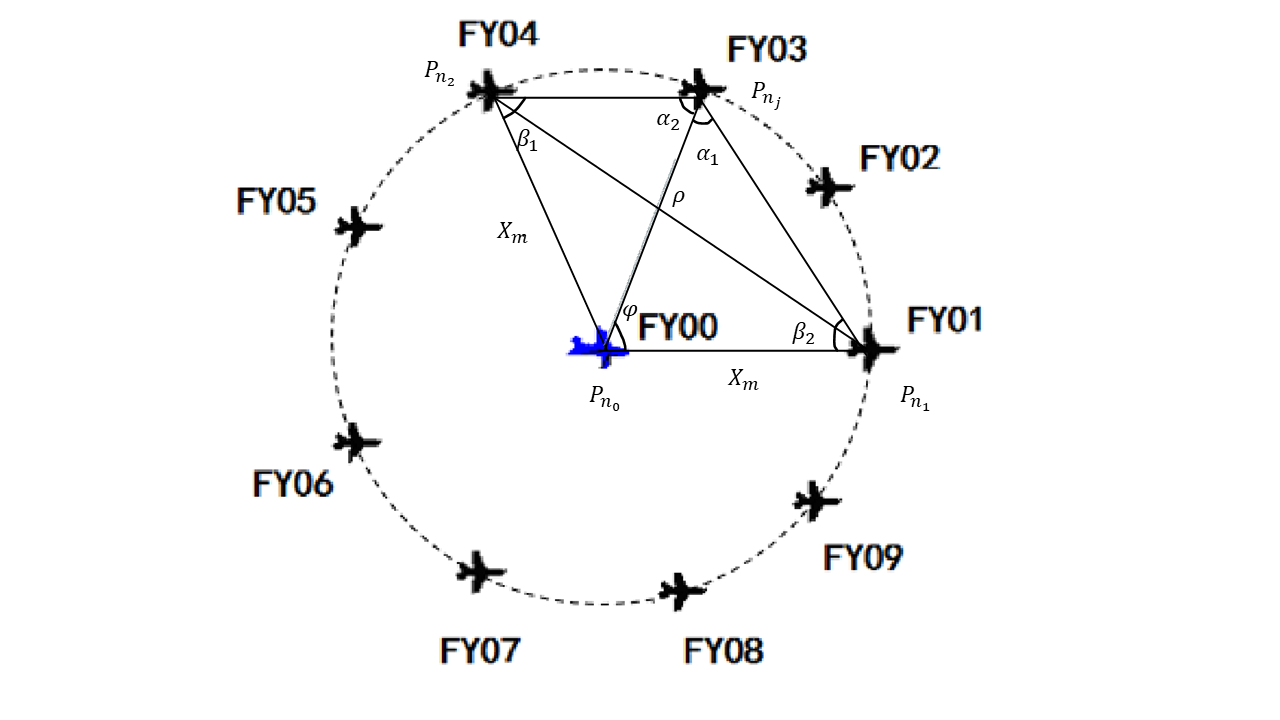
\includegraphics[width=0.6\textwidth]{1}
		\caption{圆心飞机在中间的情况}
		\label{1}
	\end{figure}
	\textcircled{1}当$\alpha_3>\alpha_1$且$\alpha_3>\alpha_2$时,如图\ref{1}:设$\angle P_{n_j}P_{n_2}P_{n_0}=\beta_1$,$\angle P_{n_0}P_{n_1}P_{n_j}=\beta_2$,$\angle P_{n_1}P_{n_0}P{n_j}=\psi$,根据正弦定理有
	$$\frac{X_m}{sm\alpha_2}=\frac{\rho}{sm\beta_1},$$ 
	$$\frac{X_m}{sm\alpha_1}=\frac{\rho}{sm\beta_2},$$
	角的关系有
	$$\beta_1 +\beta_2 +\alpha_1+\alpha_2+f(\theta )=2\pi,$$ 
	其中$f(\theta )$为圆心角,计算公式为
	$$f(\theta)=\left\{\begin{matrix} 
	\frac{\pi n}{180} (n_2-n_1),n_1<n_j<n_2  \\  
	2\pi-\frac{\pi n}{180} (n_2-n_1),n_j>n_2
	\end{matrix}\right.$$   
	上述四个方程中有三个未知数,可以解出$\rho$,$\beta_1$,$\beta_2$.在此基础上很容易求得$\theta$的值
	$$\alpha_1+\beta_2+\psi=\pi$$
	$$\theta=\frac{2}{9} \pi \times n_1+\psi $$ 
	由以上方程即可解出$\rho$,$\theta$的值。
	\begin{figure}[H]
		\centering
		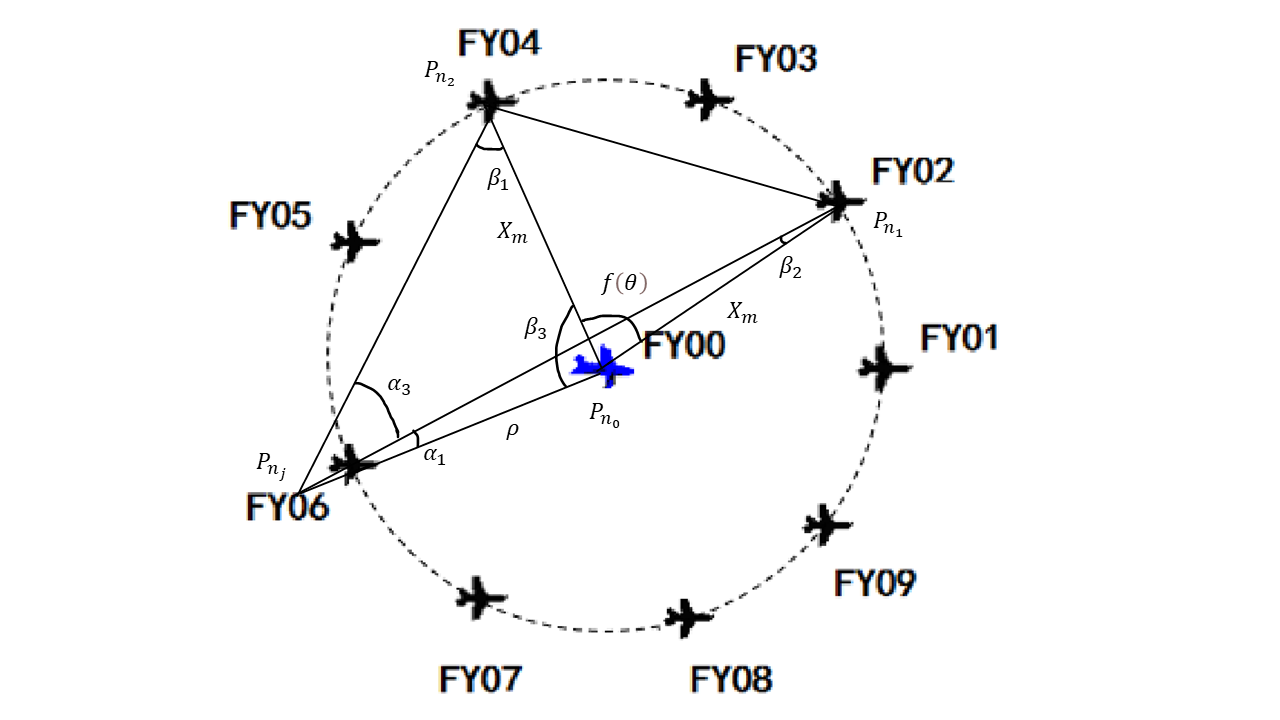
\includegraphics[width=0.6\textwidth]{2}
		\caption{圆心无人机在右侧的情况}
		\label{2}
	\end{figure}
	\textcircled{2}当$\alpha_2>\alpha_1$且$\alpha_2>\alpha_3$时,如图\ref{2}:设$\angle P_{n_j}P_{n_2}P_{n_0}=\beta_1, \angle P_{n_0}P_{n_1}P_{n_j}=\beta_2,
	\angle P_{n_1}P_{n_0}P_{n_j}=\psi$,根据正弦定理有
	$$\frac{X_m}{sm(\alpha_1+\alpha_3)}=\frac{\rho}{sm\beta_2}  $$
	$$\frac{X_m}{sm\alpha_1}=\frac{\rho}{sm\beta_1}$$
	角的关系有
	$$\beta_1+\beta_3+\alpha_1+\alpha_3=\pi$$
	$$	\alpha_1+\beta_3+ f(\theta)+\beta_2=\pi$$
	其中$f(\theta )$为圆心角,计算公式为
	$$f(\theta)=\left\{\begin{matrix} 
	\frac{\pi n}{180} (n_2-n_1),n_1<n_j<n_2  \\  
	2\pi-\frac{\pi n}{180} (n_2-n_1),n_j>n_2
	\end{matrix}\right.$$  
	上述五个方程中有三个未知数,可以解出$\rho$,$\beta_1$,$\beta_2$.在此基础上很容易求得$\theta$的值
	$$\alpha_1 + \beta_2 + \psi=\pi$$
	$$\theta=\frac{2}{9} \pi \times n_1+\psi$$
	由以上方程即可解出$\rho$,$\theta$的值。
	\begin{figure}[H]
		\centering
		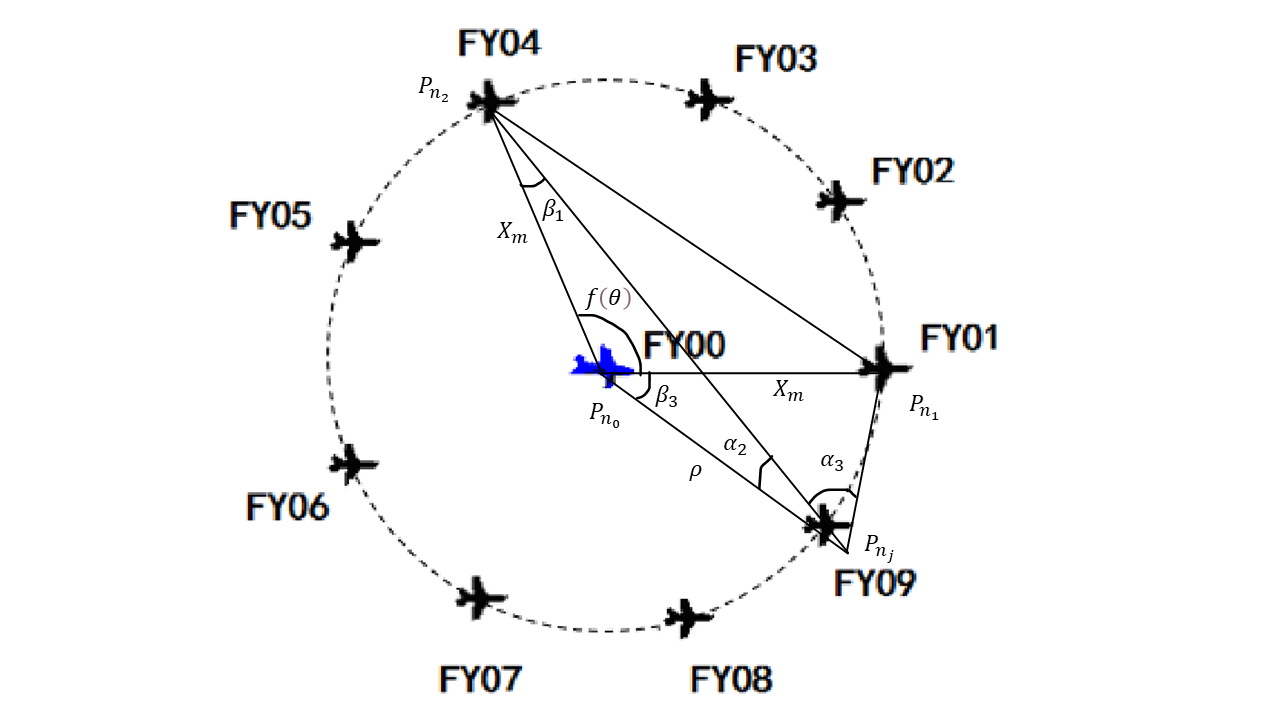
\includegraphics[width=0.6\textwidth]{3}
		\caption{圆心无人机在左侧的情况}
		\label{3}
	\end{figure}
	\textcircled{3}当$\alpha_1>\alpha_2$且$\alpha_1>\alpha_3$时,如图\ref{3}:设 $\angle P_{n_j}P_{n_2}P_{n_0}=\beta_1, \angle P_{n_0}P_{n_1}P_{n_j}=\beta_2,
	\angle P_{n_1}P_{n_0}P_{n_j}=\beta_3$,根据正弦定理有
	$$\frac{X_m}{sm(\alpha_2+\alpha_3)}=\frac{\rho}{sm\beta_2}  $$
	$$\frac{X_m}{sm\alpha_2}=\frac{\rho}{sm\beta_1}$$
	角的关系有
	$$\beta_3+\beta_1+f(\theta)+\alpha_2=\pi$$
	$$ \beta_2+\beta_3+\alpha_1+\alpha_3=\pi$$
	$$f(\theta)=\left\{\begin{matrix} 
	\frac{\pi n}{180} (n_2-n_1),n_1<n_j<n_2  \\  
	2\pi-\frac{\pi n}{180} (n_2-n_1),n_j>n_2
	\end{matrix}\right.$$  
	上述五个方程中有四个未知数,可以解出$\rho$,$\beta_1$,$\beta_2$,$\beta_3$.在此基础上很容易求得$\theta$的值
	$$ \alpha_1+\alpha_3+\beta_2+\beta_3=\psi$$
	$$\theta =\frac{2}{9}\pi \times n_1-\psi$$
	由以上方程即可解出$\rho$,$\theta$的值。
	
\subsection{问题一(2)模型的建立和求解}
若发射信号的无人机编号为$$\{n_0,n_1,n_2\},$$其中接收信号的无人机为$P_{n_j}$,假设$\alpha_1,\alpha_2$是三架飞机调整后夹角较小的两个角,现假设$P_{n_0},P_{n_1},P_{n_j}$的坐标已知,$P_{n_j}$坐标为$(x_{n_j},y_{n_j})$
\begin{figure}[H]
	\centering
	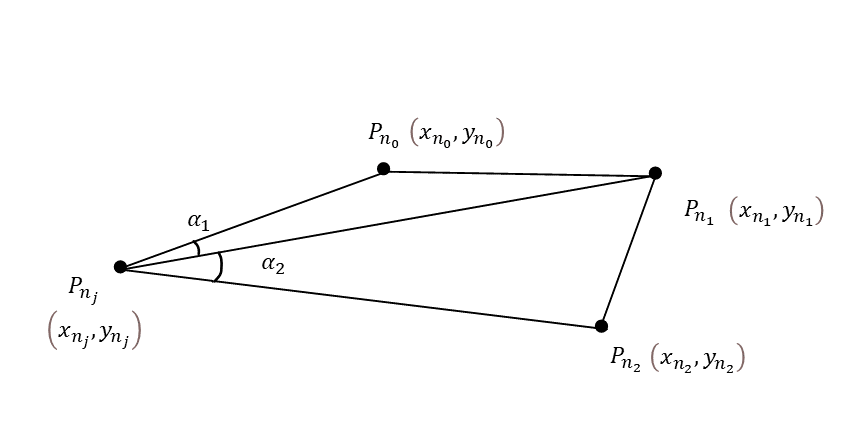
\includegraphics[width=0.5\textwidth]{4}
	\caption{两个夹角求一点}
	\label{5}
\end{figure}
对于$\alpha_1$而言,
$$\cos \alpha_1 =\frac{{(x_{n_j}-x_{n_0})^{2}}+{(x_{n_j}-x_{n_1})^{2}}+{(y_{n_j}-y_{n_0})^{2}}+{(y_{n_j}-y_{n_1})^{2}}-{(x_{n_0}-x_{n_1})^{2}}-{(y_{n_0}-y_{n_1})^{2}} }{2\sqrt{(x_{n_j}-x_{n_0})^{2}+(y_{n_j}-y_{n_0})^{2}}\times \sqrt{(x_{n_j}-x_{n_1})^{2}+(y_{n_j}-y_{n_1})^{2}}  }$$ 

同样地,对于$\alpha_2$而言,
$$\cos \alpha =\frac{{(x_{n_j}-x_{n_1})^{2}}+{(x_{n_j}-x_{n_2})^{2}}+{(y_{n_j}-y_{n_1})^{2}}+{(y_{n_j}-y_{n_2})^{2}}-{(x_{n_1}-x_{n_2})^{2}}-{(y_{n_1}-y_{n_2})^{2}} }{2\sqrt{(x_{n_j}-x_{n_1})^{2}+(y_{n_j}-y_{n_1})^{2}}\times \sqrt{(x_{n_j}-x_{n_2})^{2}+(y_{n_j}-y_{n_2})^{2}}  }$$
此时含有两个方程和两个未知数,存在解,但等式右端含有平方项,故存在多解。当无人机偏离较小时,3架无人机可有效定位。
\begin{figure}[H]
	\centering
	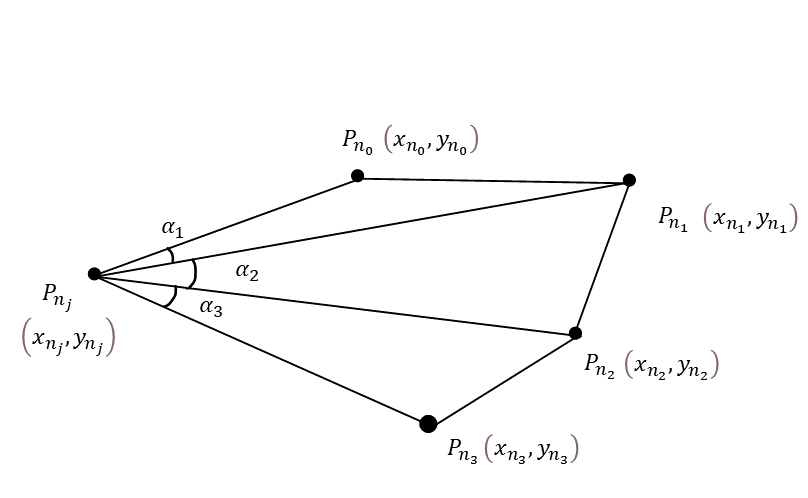
\includegraphics[width=0.5\textwidth]{5}
	\caption{三个夹角求一点}
	\label{5}
\end{figure}
未得出唯一解,在三架无人机的基础上,再加一架无人机$n_k$,设四架无人机较小的3个角为$\alpha_1,\alpha_2,\alpha_3$,则
$$\cos \alpha_3 =\frac{{(x_{n_j}-x_{n_2})^{2}}+{(x_{n_j}-x_{n_k})^{2}}+{(y_{n_j}-y_{n_2})^{2}}+{(y_{n_j}-y_{n_k})^{2}}-{(x_{n_1}-x_{n_2})^{2}}-{(y_{n_1}-y_{n_2})^{2}} }{2\sqrt{(x_{n_j}-x_{n_2})^{2}+(x_{n_j}-y_{n_2})^{2}}\times \sqrt{(x_{n_j}-x_{n_k})^{2}+(y_{n_j}-y_{n_k})^{2}}  }$$
由上面的3个式子可得$(x_j,y_j)$的唯一解,因此除了$FY00,FY01$至少还需要两架无人机才能实现接收信号无人机的有效定位.



\subsection{问题一(3)模型的建立和求解}
\subsubsection{角度分析}
圆具有很好的几何性质,现假设所有无人机的位置都没有偏差,首先对圆心无人机和圆上一架无人机发射信号,其余无人机接收信号的角度进行分析。
\begin{figure}[H]
	\centering
	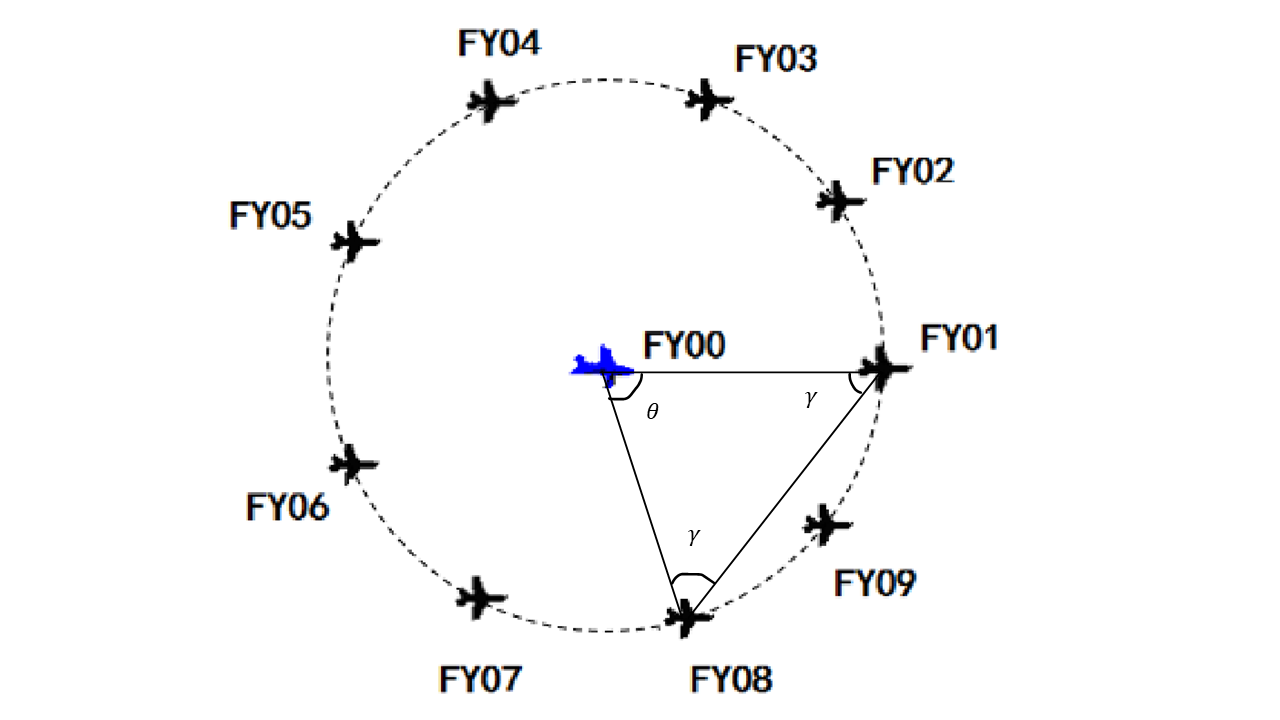
\includegraphics[width=0.6\textwidth]{6}
	\caption{圆上一架无人机的情形}
	\label{6}
\end{figure}
假设发射信号的无人机编号为$N_1=\{ n_{0},n_{1},n_{2}\},$其中$n_0=0,n_1<n_2$,圆外两架无人机的夹角为$\theta$,此时$$\alpha = \frac{\pi n}{180} (n_2-n_1),$$其中$n$代表圆周上的无人机数量,根据等腰三角形的性质,得$$\gamma=\frac{\pi-\theta}{2},$$由此可以得夹角的集合为$$\begin{bmatrix}
	10 ,& 30, & 50, & 70
\end{bmatrix}$$
\begin{figure}[H]
	\centering
	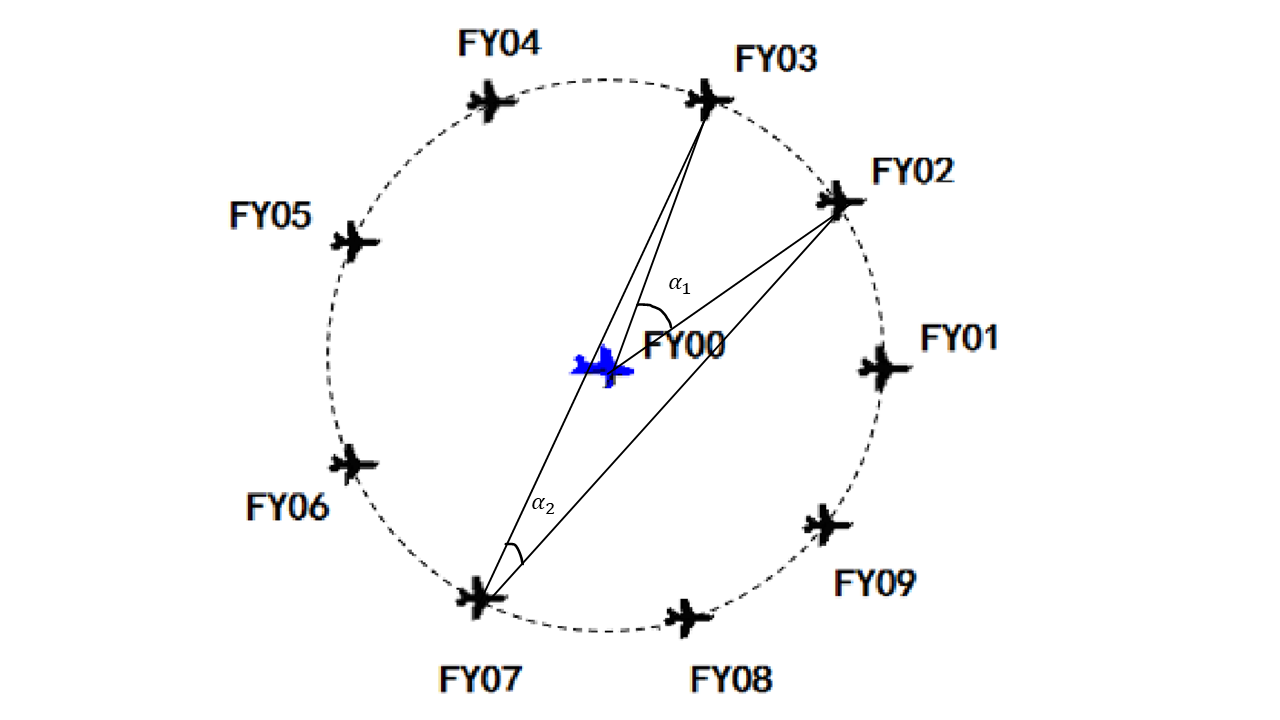
\includegraphics[width=0.6\textwidth]{7}
	\caption{圆上两架无人机的情形}
	\label{7}
\end{figure}
然后分析圆上有两架无人机的情形,圆上有两架无人机时,包含了刚才讨论的情形,因此只需要讨论圆上任意三架无人机的角度即可,发射信号的无人机编号为$N_1=\{ n_{0},n_{1},n_{2}\},$其中$n_0=0,n_1<n_2$,圆外两架无人机的夹角为$\alpha_1$,此时$$\alpha_1 = \frac{\pi n}{180},$$由于同一段弧长对应的圆周角是圆心角的一半,因此
$$\alpha_2 = \frac{\alpha_1}{2},$$由此可以得$\alpha_2$的集合为$$\begin{bmatrix}
10 ,& 20, & 30,& 40,& 50 ,& 60,&70, &80
\end{bmatrix}$$
易知,当发射信号的无人机更多时,和圆上有两架无人机的情形是一样的。通过分析发现,接收信号的无人机与圆上任意两架无人机的夹角是固定的,因此,当实际夹角的误差在$(-5\%,5\%)$之间时,可以使用k-means聚类方法调整无人机的角度。
\subsubsection{基于K-means聚类的无人机编队角度自适应调整模型}
k-means算法属于聚类算法,是一种典型的无监督学习算法。“k”表示聚类的个数,“means”意味着算法是以平均值来寻找聚类的中心的。

k-means算法的主要思想和原理为,首先从数据中随机找到k个中心,按照点到中心的距离大小,将其归为其中一类,接着每一次聚类完成后重新计算各个类的几何中心,然后重新归类,如此循环,直到最终所有类的中心不再改变为止。此时所有的数据都成功聚类。

建立了K-mean聚类方法之后,就可以调整接收信号的无人机的角度,建立模型之后使用计算机仿真,仿真过程中需要使用问题一(2)中求解调整后坐标的模型,已经证明了三个角可以确定唯一的解,但是由于误差的累积和计算机表示数值的误差,三架无人机时计算机难于求解,为了验证模型,我们采用两架无人机的模型求解。


\subsubsection{模型结果与检验}
通过计算机仿真的结果如下:
\begin{figure}[H]
	\centering
	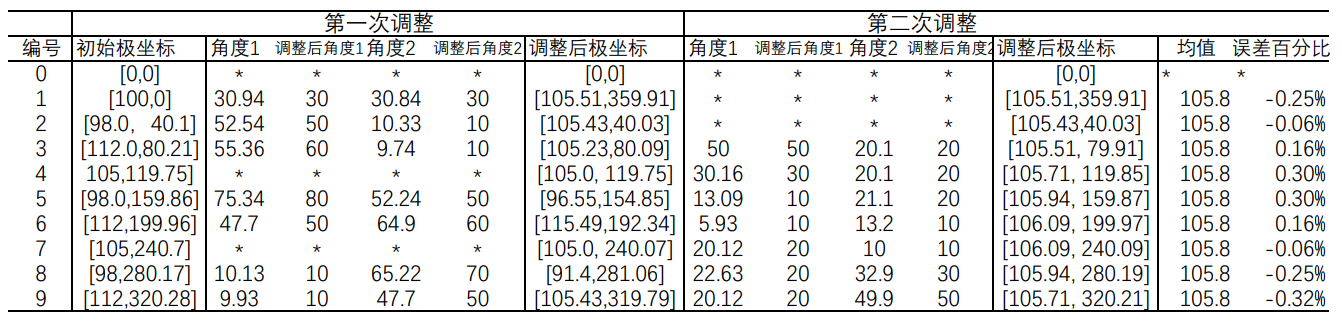
\includegraphics[width=1\textwidth]{8}
	\caption{调整过程}
	\label{8}
\end{figure}
从结果可以看出,仅需要两次调整即可,调整后的无人机均匀分布在半径为$105.77m$的圆周上,并且最大误差为$-0.32\%$,平均误差为$4.476 \times 10^{-17}$,可以认为无人机均匀分布在圆周两侧。
\subsection{问题二模型的建立和求解}
首先建立以编号为$FY13$的无人机的直角坐标系,无人机之间的距离设置为$50m$,求出每一架无人机的坐标,经过分析,当选取锥形内部三架无人机发射信号时,飞机间的角度只有三种情况$$\begin{bmatrix}
0 ,& 19.11, & 30
\end{bmatrix},$$因此假设编号为$FY05,FY08,FY09$的飞机位置是准确无误的,然后对其它接收信号的无人机加以5\%的噪声,建立基于K-means聚类的无人机编队角度自适应调整模型,计算机的仿真结果如下:
\begin{figure}[H]
	\centering
	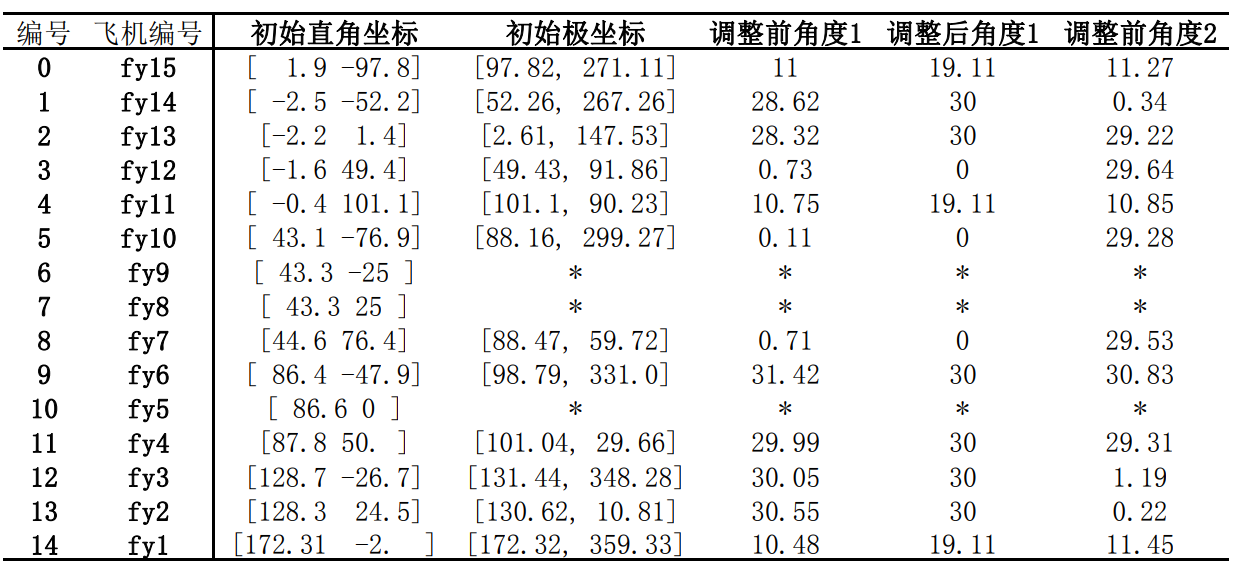
\includegraphics[width=0.99\textwidth]{9}
	\caption{调整过程}
	\label{9}
\end{figure}
通过模型易知,仅调整一次即可将接收信号的无人机调整到正确位置上。
\subsubsection{灵敏性分析}
问题一(2)中已经证明了圆上三架无人机定位时可以确定唯一的解,但是由于误差的累积和计算机表示数值的误差,圆上三架无人机定位时计算机难于求解,因此圆上三架无人机定位时不受误差的影响,而圆上两架无人机定位时对飞机偏离的程度敏感,因此我们分析锥形编队队形下对误差的敏感度,使用计算机得出以下结果:
\begin{figure}[H]
	\centering
	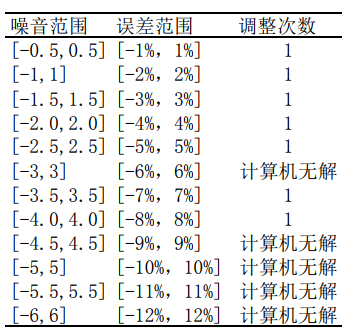
\includegraphics[width=0.5\textwidth]{10}
	\caption{模型对误差的敏感度}
	\label{10}
\end{figure}
从结果可以看出,当误差小于5\%,模型具有良好的性能,当误差超过5\%时,模型鲁棒性下降,超过10\%,时模型性能大幅下降。
	
	
	\section{模型的评价}
\subsection{模型的优点}
\begin{itemize}
	\item 模型简单,无人机调整次数少;
	\item 无人机仅仅只需要角度就可以调整自身位置;
	\item 发射信号的无人机数量少。
\end{itemize}
\subsection{模型的缺点}

\begin{itemize}
	\item 模型依赖于初值的影响较大;
	\item 使用圆上两架无人机定位时要求飞机的误差在$(-5\%,5\%)$;
\end{itemize}

\subsection{模型的改进与推广}
\begin{itemize}
	\item 改进三架无人机时计算机的求解方法,消除对无人机偏离造成的误差影响;
	\item 模型开始时随机选定无人机发射信号。减少模型开始时指定发射信号无人机的人为干扰。
\end{itemize}
	
	
		\begin{thebibliography}{9}%宽度9
			\bibitem{3}杨盛庆. 基于几何力学与最优控制的无人机编队方法研究[D].北京理工大学,2014.
		\end{thebibliography}
	
	%\section{参考文献}
	%\addcontentsline{toc}{section}{参考文献}
	\nocite{*}
	\bibliographystyle{gbt7714-numerical}
	%\bibliographystyle{unsrt}
	%\bibliographystyle{IEEEtran}
	
	\newpage
	%附录
	\begin{appendices}
		\section{文件列表}
		% Table generated by Excel2LaTeX from sheet 'Sheet1'
		\begin{table}[htbp]
			\centering
			\caption{Add caption}
			\begin{tabularx}{\textwidth}{@{}c *1{>{\centering\arraybackslash}X}@{}}
				\toprule[1.5pt]
				文件名   & 文件描述 \\
				\midrule
				圆形编队求解.py & 圆形编队求解模型代码 \\
				锥形编队求解.py & 锥形编队求解模型代码 \\
				圆形编队求解数据.xlsx & 圆形编队求解数据 \\
				锥形编队求解数据.xlsx & 锥形编队求解数据 \\
				锥形模型敏感度分析结果.xlsx & 锥形模型敏感度分析结果 \\
				\bottomrule
			\end{tabularx}%
			\label{tab:addlabel}%
		\end{table}%
		
		
		\section{代码}
		圆形编队求解.py
		\lstinputlisting[language=python]{code/1.py}
		锥形编队求解.py
		\lstinputlisting[language=python]{code/2.py}
		

	\end{appendices}
	
\end{document} 